\documentclass[conference]{IEEEtran}
% \IEEEoverridecommandlockouts
% The preceding line is only needed to identify funding in the first footnote. If that is unneeded, please comment it out.
%Template version as of 6/27/2024

\usepackage[noadjust]{cite}
\usepackage{amsmath,amssymb,amsfonts}
\usepackage{algorithmic}
\usepackage{graphicx}
\usepackage{textcomp}
\usepackage{xcolor}
\def\BibTeX{{\rm B\kern-.05em{\sc i\kern-.025em b}\kern-.08em
    T\kern-.1667em\lower.7ex\hbox{E}\kern-.125emX}}
\begin{document}

\title{Sintetizando episódios de treino via abstração de jogos em aprendizado por reforço}

\author{\IEEEauthorblockN{Marcelo Augusto Salomão Ganem}
\IEEEauthorblockA{\textit{Departamento de Ciência da Computação (UFMG)} \\
Belo Horizonte, Minas Gerais \\
marceloganem@dcc.ufmg.br}
}

\maketitle

\begin{abstract}
This document is a model and instructions for \LaTeX.
This and the IEEEtran.cls file define the components of your paper [title, text, heads, etc.]. *CRITICAL: Do Not Use Symbols, Special Characters, Footnotes, 
or Math in Paper Title or Abstract.
\end{abstract}

\begin{IEEEkeywords}
    reinforcement learning, game modeling, board games, curriculum learning
\end{IEEEkeywords}

\section{Introdução}
\label{intro}
Um desafio central abordado pela literatura de aprendizado por reforço há mais de duas décadas é a combinação de planejamento e aprendizado de maneira a minimizar a necessidade de intervenções humanas e maximizar a generalização dos comportamentos obtidos. Dentre as formas mais tradicionais de introduzir estrutura a partir de conhecimento especializado em soluções de aprendizado por reforço está a construção de \textit{features} que sejam uma abstração suficientemente representativa do ambiente apresentado ao agente. 

Especificamente no domínio de jogos (virtuais e de tabuleiro), um obstáculo frequentemente encontrado é a complexidade de regras e relações que precisam ser implicitamente compreendidas pelo agente. Mesmo que triviais para humanos, a combinação de um conjunto de regras suficientemente ortogonais entre si é capaz de produzir dinâmicas e estados com padrões ruidosos que, quando não explicados por um conjunto de regras explícitas, demandam aproximadores de funções complexos e treinamento extensivo para serem identificados.

Joris Dormans\cite{machinations} investiga a produção do chamado comportamento emergente em jogos, propondo uma sintaxe relativamente simples capaz de evidenciar os recursos e entidades centrais em um jogo, bem como as relações entre essas entidades. Assim, de acordo com Dormans, é possível rapidamente identificar ciclos de retroalimentação que ditam a economia geral de um jogo.

Os diagramas construídos pela sintaxe proposta, enquanto conceitualmente sob domínio público, não estão mais publicamente disponíveis para teste e simulação -- a empresa Machinations SARL\footnote{Link about} atualmente oferece esse serviço de maneira privada a empresas de desenvolvimento e design de jogos. Ao longo da última década, publicações pontuais exploraram a aplicabilidade das proposições de Dormans no contexto de computação.\footnote{Outro link publications}


\section{Objetivos}
\label{goals}

O presente trabalho visa, portanto, construir uma representação simplificada e formalizada de diagramas  Machinations para representar um conjunto amplo de jogos compreendidos pela combinação dos elementos e conexões disponíveis. 

A partir disso, investigamos a aplicabilidade dessas representações simplificadas no treino de agentes de aprendizado por reforço como uma pré-otimização com respeito à verdadeira política ótima -- dentre as múltiplas formas de utilizar a riqueza semântica e estrutural dessas representações na construção de modelos de IA.

\section{Trabalhos Relacionados}
A hipótese aqui investigada se sustenta centralmente, além de em conceitos da literatura geral de aprendizado por reforço, em trabalhos que propõem, viabilizam e justificam a utilização de representações abstrativas e simplificadas para pelo menos parte do aprendizado.

\subsection{Engineering Emergence}
\label{references:machinations}
O elemento central do trabalho "\textit{Engineering Emergence: Applied Theory for Game Design}"\cite{machinations} é a definição de uma gramática de elementos para a composição de uma estrutura semelhante a um grafo cuja premissa é representar o estado da economia interna de um jogo.
\begin{figure}[h!]
    \centering
    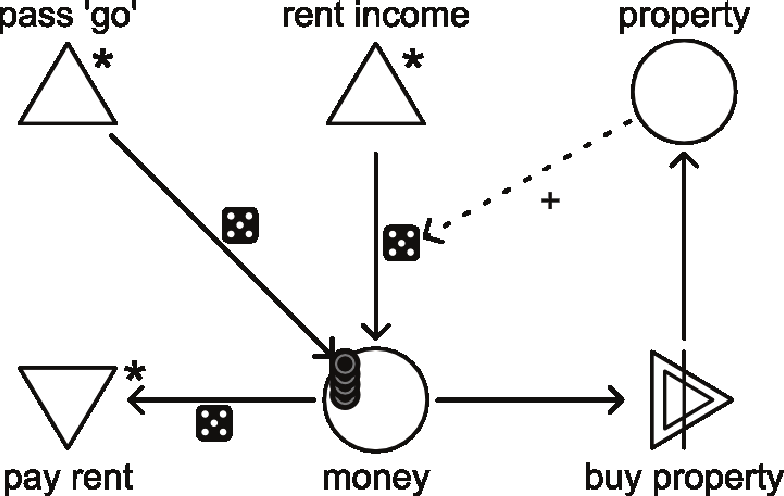
\includegraphics[width=0.9\linewidth]{figures/monopoly.png}
    \caption{Representação do jogo \textit{Monopoly} sob a sintaxe \textit{Machinations}}.
    \label{fig:monopoly}
\end{figure}

O autor define essa economia interna como a alocação dos recursos (representados na Figura \ref{fig:monopoly} como fichas em cima de cada nó) entre os nós. O estado dessa economia é alterado a partir do andamento discreto do tempo e ações do jogador ou de quaisquer agentes presentes no sistema. O caráter dessas transições, i.e., o estado atingido em seguida, é ditado pelas arestas do grafo, que indicam transferência regular, condicional ou probabilística de recursos.

Como mencionado na Seção \ref{goals}, visamos construir uma versão formal e simplificada dos elementos e regras propostas por Dormans. A Seção \ref{modeling} se dedica à transcrição das definições originais para o contexto de um Processo de Decisão de Markov (MDP) adequado para aprendizado por reforço.

\subsection{Curriculum Learning}
A premissa de que um agente é capaz de aprender uma representação útil da política ótima no problema final a partir de uma versão simplificada de um problema é firmada no conceito de curriculum learning. Especificamente, Bengio et al.\cite{curriculum} formalizam a intuição de que apresentar tarefas de dificuldade crescente em ordem durante o treinamento de um agente é mais efetivo do que apresentar o problema completo.

Nesse sentido, o treinamento de um agente de aprendizado por reforço em um diagrama Machinations suficientemente representativo pode ser visto como uma otimização não-refinada com respeito ao problema original. Naturalmente, essa premissa é sensível à qualidade da representação abstrata, i.e., o quanto a dinâmica do problema original apresenta um comportamento coerente em comparação à dinâmica simplificada.

\subsection{Relational Reinforcement Learning}
Tadepalli et al. \cite{rrl} investigaram há mais de duas décadas a relevância da ideia de representações relacionalmente estruturadas no contexto de aprendizado por reforço. Especificamente, os autores observam que diversas das técnicas de aprendizado por reforço apresentadas à época -- de fato, grande parte das técnicas de aprendizado por reforço até hoje -- introduziam informações semanticamente relacionais sobre o problema de formas diferentes.

A introdução de diagramas Machinations como um ambiente de treino pode ser vista como mais um caso da observação feita: primeiro, o agente é exposto a um ambiente que compreende estritamente os elementos centrais da economia de um jogo e que se comporta conforme as relações mais significativas entre eles. Observando o estado do diagrama, de dimensionalidade tipicamente inferior a representações reais (sobretudo de jogos virtuais), o aprendizado necessário é essencialmente da relação numérica entre as variáveis observadas -- e quais delas estão correlacionadas a recompensas positivas e negativas.

\subsection{A modeling environment for reinforcement learning in games}
"A modeling environment for reinforcement learnig in games" coincide com o presente trabalho na busca por uma solução genérica e explicável para a produção consistente e controlável de comportamentos artificialmente inteligentes. Gomes et al.\cite{modeling-rl-games} declaram um objetivo muito semelhante:
\begin{quote}
    Thus, AI4U was specifically refined to the preparation of reinforcement learning experiments in games. In general, the high-level goals of this environment are: to enable the reproducibility of methods and results; \textbf{to simplify the way of designing reinforcement learning algorithms in games;} and to enhance the readability of RL agents.
\end{quote}

A solução apresentada pelos autores se centraliza na definição de uma ontologia de elementos e comportamentos compatíveis com definições comuns em engines de jogos, tal que desenvolvedores são capazes de especificar elementos das interações e regras desejadas para reforçar comportamentos em personagens não jogáveis. Observamos, assim, uma evidência da eficácia da introdução de uma simplificação relacional estruturada como linguagem única para a produção de uma solução em aprendizado por reforço.

\section{Metodologia}

O problema proposto é abordado primeiro pela modelagem dos elementos e regras universais a todas as simulações simplificadas sob o prisma de um MDP. Então, modelamos os jogos Blackjack e Monopoly para verificar a capacidade do novo conjunto de definições básicas. Por fim, aplicamos Proximal Policy Optimization ao cenário simulado do Monopoly para verificar a capacidade de convergência do agente para a política ótima no cenário proposto.

As dificuldades enfrentadas na parte de aprendizado, elaboradas na Seção \ref{results}, dificultam a extensão dos agentes treinados nas simulações para o problema real. Dedicamos este estudo, portanto, à investigação das propriedades dos diagramas implementados no contexto de aprendizado por reforço, bem como dos obstáculos encontrados.

\subsection{Modelagem}
\label{modeling}
Machinations

\subsubsection{Ações}

Powerset of nodes

$$
aaaaa
$$

\subsubsection{Estados}

Estados dos nos e conexoes de recursos
Subconjunto dos estados visiveis

\subsubsection{Dinâmica}

literalmente as regras do bagui

\subsubsection{Recompensas}

Pesos para cada um dos elementos observáveis, +1 quando ganha, só conta pesos negativos quando perde.

\subsection{Jogos modelados}
bla bla bla geral \footnote{Explicando porque nao estamos indo com o Catan...}
\subsubsection{Blackjack}
\subsubsection{Monopoly}
This environment should produce the classic monopoly dilemma: "I need to invest to survive long-term, but investing makes me vulnerable short-term"


Monopoly é o jogo no qual vamos testar a aplicabilidade de RL (por ser o mais explicitamente definido no trabalho de referência, além de que são problemas completamente diferentes com técnicas de aprendizado completamente diferentes... melhor se dedicar a explorar um só). Além disso, o blackjack acaba tendo o diagrama mais complexo que a modelagem.

\subsection{Aprendizado}
DQN -> por quê? 
Quais parâmetros? Quantos episódios?
\begin{quote}
    \small
    \color{blue}
    learning rate=0.0005,            (Reduced from 1e-3 for stability)
    buffer size=100000,              (Increased from 50000 for better experience replay)
    learning starts=5000,            (Reduced from 10000 for faster learning with short episodes)
    batch size=256,                  (Increased from 64 for smoother gradient updates)
    gamma=0.95,                      (Reduced from 0.99 for shorter episode focus)
    train freq=1,                    (Increased from 4 for more frequent updates)
    gradient steps=1,
    target update interval=5000,     (Increased from 1000 to prevent instability)
    exploration fraction=0.3,        (Reduced from 0.5 for faster convergence)
    exploration initial eps=1.0,
    exploration final eps=0.05,      (Increased from 0.01 to maintain exploration)
\end{quote}
Spoiler: DQN Falhou... falar mais em resultados.

\section{Resultados}
\label{results}
DQN falhou por uma pá de coisa:

\begin{quote}
    \small
    \color{blue}
    DQNs are fundamentally ill-suited for this highly stochastic monopoly environment. Here's why:
    Core Stochastic Challenges
    70\% chance to pay rent each step (pay rent odds: luck ≤ 28 out of 40)
    25x rent variance (\$2-50 from rent values array)
    17.5\% chance of income (pass go odds: luck ≤ 7 out of 40)
    35\% chance of rent income (get rent odds: luck ≤ 14 out of 40)

    Why DQNs Fail Here
    1. High Variance Breaks Q-Learning
    DQNs learn expected Q-values, but with 25x rent variance, the same state-action pair can yield vastly different outcomes
    A "good" action (buying estates) can still lead to immediate bankruptcy due to bad luck
    Q-values become unreliable when signal-to-noise ratio is this poor
    2. Sparse Binary Rewards
    The environment gives mostly -1 (bankruptcy) or +1 (survival) with little intermediate feedback
    DQNs need dense reward signals to understand which actions contribute to success
    With binary outcomes, it's nearly impossible to distinguish good vs bad actions from limited samples
    3. Stochastic Transitions Violate DQN Assumptions
    DQNs assume actions have somewhat predictable consequences
    Here, even optimal actions can fail due to multiple layers of randomness
    The Markov property is weakened when outcomes depend heavily on unobservable luck
    4. Sample Inefficiency
    Your evaluation shows mean episode length of only 8.9 steps before bankruptcy
    DQNs need thousands of episodes, but short episodes provide minimal learning signal
    Most episodes end the same way (bankrupt) regardless of strategy

\end{quote}

Pra um jogo o trabalho de referência não serve devido a problemas de desambiguação temporal. Além disso, a gente vê que a modelagem em si acaba sendo mais complexa que o próprio jogo. no outro o agente converge pra um ótimo local de sempre comprar.

\section{Considerações}

\section{Trabalhos futuros}


\newpage

\section{Introduction}
This document is a model and instructions for \LaTeX.
Please observe the conference page limits. For more information about how to become an IEEE Conference author or how to write your paper, please visit   IEEE Conference Author Center website: https://conferences.ieeeauthorcenter.ieee.org/.

\subsection{Maintaining the Integrity of the Specifications}

The IEEEtran class file is used to format your paper and style the text. All margins, 
column widths, line spaces, and text fonts are prescribed; please do not 
alter them. You may note peculiarities. For example, the head margin
measures proportionately more than is customary. This measurement 
and others are deliberate, using specifications that anticipate your paper 
as one part of the entire proceedings, and not as an independent document. 
Please do not revise any of the current designations.

\section{Prepare Your Paper Before Styling}
Before you begin to format your paper, first write and save the content as a 
separate text file. Complete all content and organizational editing before 
formatting. Please note sections \ref{AA} to \ref{FAT} below for more information on 
proofreading, spelling and grammar.

Keep your text and graphic files separate until after the text has been 
formatted and styled. Do not number text heads---{\LaTeX} will do that 
for you.

\subsection{Abbreviations and Acronyms}\label{AA}
Define abbreviations and acronyms the first time they are used in the text, 
even after they have been defined in the abstract. Abbreviations such as 
IEEE, SI, MKS, CGS, ac, dc, and rms do not have to be defined. Do not use 
abbreviations in the title or heads unless they are unavoidable.

\subsection{Units}
\begin{itemize}
\item Use either SI (MKS) or CGS as primary units. (SI units are encouraged.) English units may be used as secondary units (in parentheses). An exception would be the use of English units as identifiers in trade, such as ``3.5-inch disk drive''.
\item Avoid combining SI and CGS units, such as current in amperes and magnetic field in oersteds. This often leads to confusion because equations do not balance dimensionally. If you must use mixed units, clearly state the units for each quantity that you use in an equation.
\item Do not mix complete spellings and abbreviations of units: ``Wb/m\textsuperscript{2}'' or ``webers per square meter'', not ``webers/m\textsuperscript{2}''. Spell out units when they appear in text: ``. . . a few henries'', not ``. . . a few H''.
\item Use a zero before decimal points: ``0.25'', not ``.25''. Use ``cm\textsuperscript{3}'', not ``cc''.)
\end{itemize}

\subsection{Equations}
Number equations consecutively. To make your 
equations more compact, you may use the solidus (~/~), the exp function, or 
appropriate exponents. Italicize Roman symbols for quantities and variables, 
but not Greek symbols. Use a long dash rather than a hyphen for a minus 
sign. Punctuate equations with commas or periods when they are part of a 
sentence, as in:
\begin{equation}
a+b=\gamma\label{eq}
\end{equation}

Be sure that the 
symbols in your equation have been defined before or immediately following 
the equation. Use ``\eqref{eq}'', not ``Eq.~\eqref{eq}'' or ``equation \eqref{eq}'', except at 
the beginning of a sentence: ``Equation \eqref{eq} is . . .''

\subsection{\LaTeX-Specific Advice}

Please use ``soft'' (e.g., \verb|\eqref{Eq}|) cross references instead
of ``hard'' references (e.g., \verb|(1)|). That will make it possible
to combine sections, add equations, or change the order of figures or
citations without having to go through the file line by line.

Please don't use the \verb|{eqnarray}| equation environment. Use
\verb|{align}| or \verb|{IEEEeqnarray}| instead. The \verb|{eqnarray}|
environment leaves unsightly spaces around relation symbols.

Please note that the \verb|{subequations}| environment in {\LaTeX}
will increment the main equation counter even when there are no
equation numbers displayed. If you forget that, you might write an
article in which the equation numbers skip from (17) to (20), causing
the copy editors to wonder if you've discovered a new method of
counting.

{\BibTeX} does not work by magic. It doesn't get the bibliographic
data from thin air but from .bib files. If you use {\BibTeX} to produce a
bibliography you must send the .bib files. 

{\LaTeX} can't read your mind. If you assign the same label to a
subsubsection and a table, you might find that Table I has been cross
referenced as Table IV-B3. 

{\LaTeX} does not have precognitive abilities. If you put a
\verb|\label| command before the command that updates the counter it's
supposed to be using, the label will pick up the last counter to be
cross referenced instead. In particular, a \verb|\label| command
should not go before the caption of a figure or a table.

Do not use \verb|\nonumber| inside the \verb|{array}| environment. It
will not stop equation numbers inside \verb|{array}| (there won't be
any anyway) and it might stop a wanted equation number in the
surrounding equation.

\subsection{Some Common Mistakes}\label{SCM}
\begin{itemize}
\item The word ``data'' is plural, not singular.
\item The subscript for the permeability of vacuum $\mu_{0}$, and other common scientific constants, is zero with subscript formatting, not a lowercase letter ``o''.
\item In American English, commas, semicolons, periods, question and exclamation marks are located within quotation marks only when a complete thought or name is cited, such as a title or full quotation. When quotation marks are used, instead of a bold or italic typeface, to highlight a word or phrase, punctuation should appear outside of the quotation marks. A parenthetical phrase or statement at the end of a sentence is punctuated outside of the closing parenthesis (like this). (A parenthetical sentence is punctuated within the parentheses.)
\item A graph within a graph is an ``inset'', not an ``insert''. The word alternatively is preferred to the word ``alternately'' (unless you really mean something that alternates).
\item Do not use the word ``essentially'' to mean ``approximately'' or ``effectively''.
\item In your paper title, if the words ``that uses'' can accurately replace the word ``using'', capitalize the ``u''; if not, keep using lower-cased.
\item Be aware of the different meanings of the homophones ``affect'' and ``effect'', ``complement'' and ``compliment'', ``discreet'' and ``discrete'', ``principal'' and ``principle''.
\item Do not confuse ``imply'' and ``infer''.
\item The prefix ``non'' is not a word; it should be joined to the word it modifies, usually without a hyphen.
\item There is no period after the ``et'' in the Latin abbreviation ``et al.''.
\item The abbreviation ``i.e.'' means ``that is'', and the abbreviation ``e.g.'' means ``for example''.
\end{itemize}

\subsection{Authors and Affiliations}\label{AAA}
\textbf{The class file is designed for, but not limited to, six authors.} A 
minimum of one author is required for all conference articles. Author names 
should be listed starting from left to right and then moving down to the 
next line. This is the author sequence that will be used in future citations 
and by indexing services. Names should not be listed in columns nor group by 
affiliation. Please keep your affiliations as succinct as possible (for 
example, do not differentiate among departments of the same organization).

\subsection{Identify the Headings}\label{ITH}
Headings, or heads, are organizational devices that guide the reader through 
your paper. There are two types: component heads and text heads.

Component heads identify the different components of your paper and are not 
topically subordinate to each other. Examples include Acknowledgments and 
References and, for these, the correct style to use is ``Heading 5''. Use 
``figure caption'' for your Figure captions, and ``table head'' for your 
table title. Run-in heads, such as ``Abstract'', will require you to apply a 
style (in this case, italic) in addition to the style provided by the drop 
down menu to differentiate the head from the text.

Text heads organize the topics on a relational, hierarchical basis. For 
example, the paper title is the primary text head because all subsequent 
material relates and elaborates on this one topic. If there are two or more 
sub-topics, the next level head (uppercase Roman numerals) should be used 
and, conversely, if there are not at least two sub-topics, then no subheads 
should be introduced.

\subsection{Figures and Tables}\label{FAT}
\paragraph{Positioning Figures and Tables} Place figures and tables at the top and 
bottom of columns. Avoid placing them in the middle of columns. Large 
figures and tables may span across both columns. Figure captions should be 
below the figures; table heads should appear above the tables. Insert 
figures and tables after they are cited in the text. Use the abbreviation 
``Fig.~\ref{fig}'', even at the beginning of a sentence.

\begin{table}[htbp]
\caption{Table Type Styles}
\begin{center}
\begin{tabular}{|c|c|c|c|}
\hline
\textbf{Table}&\multicolumn{3}{|c|}{\textbf{Table Column Head}} \\
\cline{2-4} 
\textbf{Head} & \textbf{\textit{Table column subhead}}& \textbf{\textit{Subhead}}& \textbf{\textit{Subhead}} \\
\hline
copy& More table copy$^{\mathrm{a}}$& &  \\
\hline
\multicolumn{4}{l}{$^{\mathrm{a}}$Sample of a Table footnote.}
\end{tabular}
\label{tab1}
\end{center}
\end{table}

\begin{figure}[htbp]
\centerline{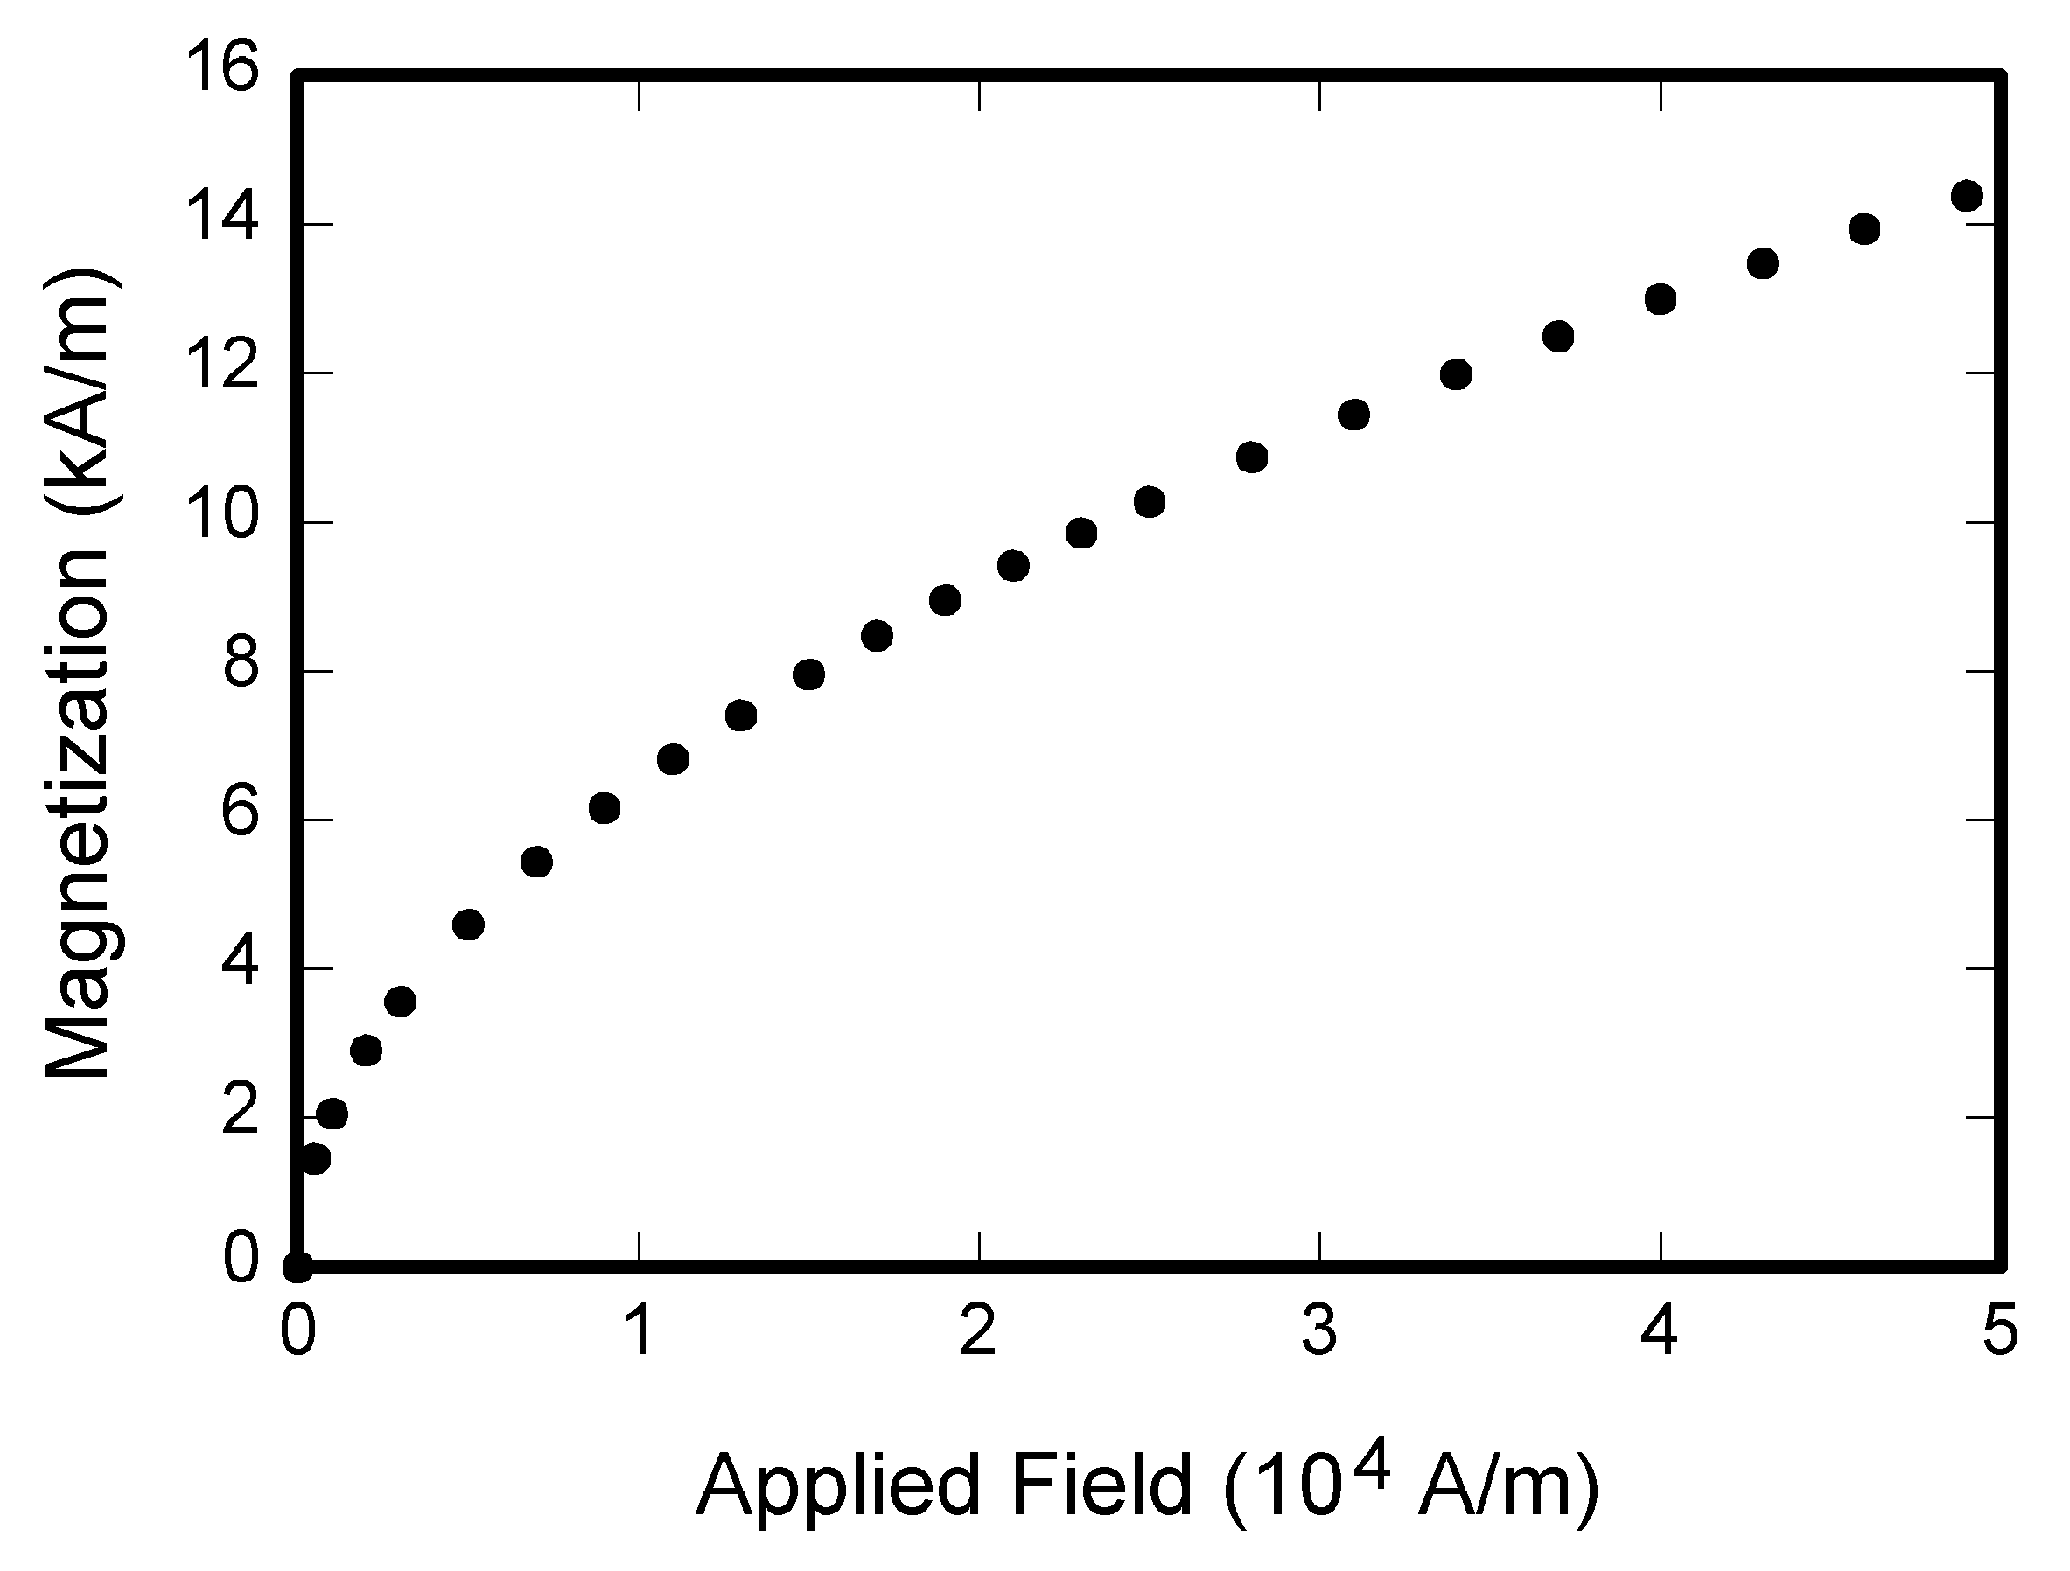
\includegraphics{fig1.png}}
\caption{Example of a figure caption.}
\label{fig}
\end{figure}

Figure Labels: Use 8 point Times New Roman for Figure labels. Use words 
rather than symbols or abbreviations when writing Figure axis labels to 
avoid confusing the reader. As an example, write the quantity 
``Magnetization'', or ``Magnetization, M'', not just ``M''. If including 
units in the label, present them within parentheses. Do not label axes only 
with units. In the example, write ``Magnetization (A/m)'' or ``Magnetization 
\{A[m(1)]\}'', not just ``A/m''. Do not label axes with a ratio of 
quantities and units. For example, write ``Temperature (K)'', not 
``Temperature/K''.

\section*{Acknowledgment}

The preferred spelling of the word ``acknowledgment'' in America is without 
an ``e'' after the ``g''. Avoid the stilted expression ``one of us (R. B. 
G.) thanks $\ldots$''. Instead, try ``R. B. G. thanks$\ldots$''. Put sponsor 
acknowledgments in the unnumbered footnote on the first page.

\section*{References}


Number footnotes separately in superscripts. Place the actual footnote at 
the bottom of the column in which it was cited. Do not put footnotes in the 
abstract or reference list. Use letters for table footnotes.

Unless there are six authors or more give all authors' names; do not use 
``et al.''. Papers that have not been published, even if they have been 
Capitalize only the first word in a paper title, except for proper nouns and 
element symbols.\cite{modeling-rl-games}

For papers published in translation journals, please give the English 

\vspace{12pt}
\bibliographystyle{IEEEtran}
\bibliography{references}
\end{document}
